\subsection{Шифр Цезаря}

Шифр Цезаря — это вид шифра подстановки, в котором каждый символ 
в открытом тексте заменяется буквой находящейся на некоторое 
постоянное число позиций левее или правее него в алфавите.

Шифр назван в честь римского императора Гая Юлия Цезаря, использовавшего 
его для секретной переписки со своими генералами.

\subsubsection{Описание}

Если сопоставить каждому символу алфавита его порядковый номер 
(нумеруя с 0), то шифрование и дешифрование можно выразить формулами 
модульной арифметики:

    $$y=(x+k)\ \mod\ n$$
    $$x=(y-k+n)\ \mod\ n,$$

где $x$ — символ открытого текста, $y$ — символ шифрованного 
текста, $n$ — мощность алфавита, а $k$ — ключ.

\subsubsection{Криптоанализ, реализация простого перебора и архитектура базового класса}

Шифр Цезаря может быть легко взломан даже в случае, когда взломщик 
знает только зашифрованный текст. Можно рассмотреть две ситуации:

\begin{enumerate}
\item Известно что использовался простой шифр подстановки, но 
    не известно, что это — схема Цезаря;
\item Известно что использовался шифр Цезаря, но не известно 
   значение сдвига.
\end{enumerate}

В первом случае шифр может быть взломан, используя те же самые 
методы что и для простого шифра подстановки — частотный 
анализ с перебором по описанным ранее лингвистическим метрикам.
Таким образом, взломщик, вероятно, быстро 
заметит регулярность в решении и поймёт, что используемый шифр — 
это шифр Цезаря.

Во втором случае, взлом шифра является даже более простым. Существует 
не так много вариантов значений сдвига (26 для английского языка), 
все они могут быть проверены методом перебора.

Для обычного текста на естественном языке, скорее всего, будет 
только один вариант декодирования. Но, если использовать очень 
короткие сообщения, то возможны случаи, когда возможны несколько 
вариантов расшифровки с различными сдвигами. Например зашифрованный 
текст MPQY может быть расшифрован как «aden» так и как «know» 
(предполагая, что открытый текст написан на английском языке). 
Точно также «ALIIP» можно расшифровать как «dolls» или как «wheel
»; «AFCCP» как «jolly» или как «cheer».

Благодаря малому количеству ключей криптоанализ сводится
к применению функции расшифрования ко всем текстам и 
поиск в результатах текста с максимальной метрикой: 

\begin{listing}[1]{1}
import cipher.cesar
def dechiper(ctext):
    c = cipher.cesar(ctext)
    scores = [(fitness.score(c.decrypt(i)), i) for i in range(26)]
    return max(scores)
\end{listing}

Относитьельно шифра Цезаря осталось добавить, что
многократное шифрование никак не улучшает стойкость, так как 
применение шифров со сдвигом $a$ и $b$ эквивалентно применению шифра 
со сдвигом $a+b$. В математических терминах шифрование с различными 
ключами образует группу.

Прешло время обсудить реализацию каждого класса в фреймворке 

\begin{figure}[h]
\noindent\centering{
    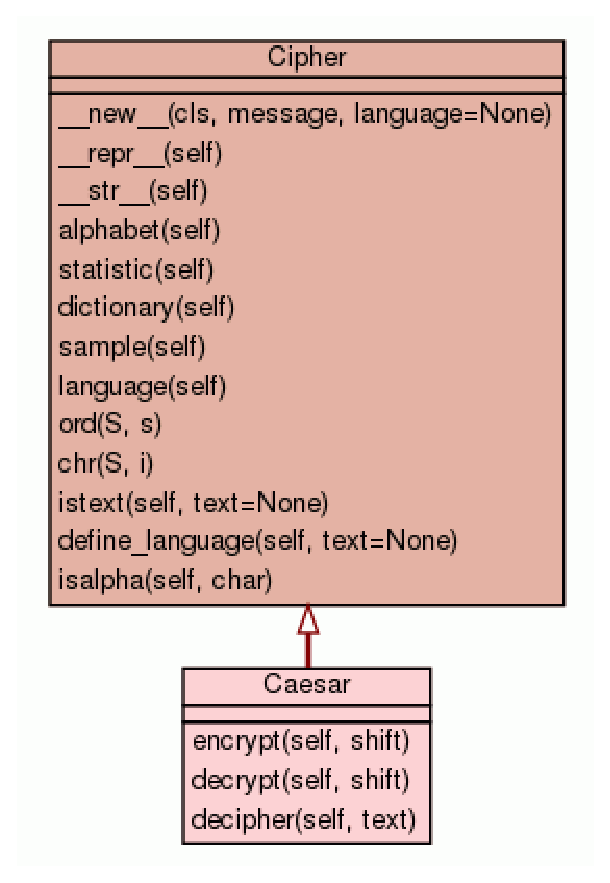
\includegraphics[width=65mm]{\globalImages/uml_cesar.eps}
}
\caption{UML диаграмма класса анализа шифра Цезаря}
\label{figUCesar}
\end{figure}


\begin{figure}[h]
\noindent\centering{
    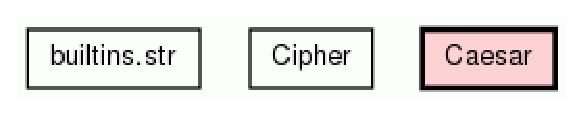
\includegraphics[width=75mm]{\globalImages/hierarchy_caesar.eps}
}
\caption{Иерархическая диаграмма класса анализа шифра Цезаря}
\label{figICesar}
\end{figure}


\begin{figure}[h]
\noindent\centering{
    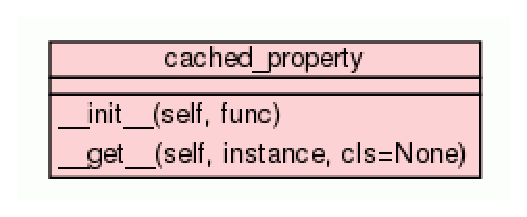
\includegraphics[width=65mm]{\globalImages/uml_cached.eps}
}
\caption{UML диаграмма класса для кеширования свойств}
\label{figCached}
\end{figure}
